\subsection{Overview}
\noindent
To comply with standard design practices it is suggested to undergo unit testing as each component is built, integration testing as components get pieced together, and system testing to validate the system as a whole. This section will detail the order in which the components should be built, the method to carry out testing, and the manner in which to integrate the components.

\subsection{Implementation Plan}
\subsubsection{DBMS}
\noindent
The structure of the database and storage servers should be implemented first. Investing in the implementation of these components first lays out the foundation of the structure of the data expected by the system before starting the implementation of the application components as described in Section \ref{sect:AppIIT}. Additionally, after the DBMS and storage components are implemented, these components can serve as a bed for continuous integration testing as the system gets incrementally built. This is explained in further detail in Section \ref{sect:ITP}. 

\subsubsection{DREAM Application}
\label{sect:AppIIT}
\noindent
As stated previously, the entire system can be decomposed into 15 components which shall be built in the following order: 

\begin{enumerate}
\item AuthenticationManager
\item FarmerReportManager
\item AgronomistReportManager
\item DataAggregationManager
\item StatisticsManager
\item DailyPlanManager
\item MessageManager
\item FarmManager
\item RankingManager
\item TriggerManager
\item NotificationManager
\item ForumManager
\item FarmerSuggestionManager
\item RecommenderManager
\item WeatherManager
\end{enumerate}

\noindent
This ordering of components prioritizes the most important features expected by the DREAM system and core components that serve as a foundation or basis for other components. Namely, the \(\ll\)AuthenticationManager\(\gg\) is the first component to be built to emphasize the importance of security. Before any user can do anything they must be able to login. Then, components supporting the generation of reports and handling the data are listed. This is a core function of the DREAM system and the foundation of the value-add of the DREAM system. After that, additional components that generate more data and support the aggregation of diverse data sources, such as \(\ll\)DailyPlanManager\(\gg\), \(\ll\)MessageManager\(\gg\), and \(\ll\)FarmManager\(\gg\), are listed. These component just build on the core functionalities that have already been established. Then, the remaining components refine the features that the DREAM system provides and fulfill the goals committed to by the system. \smallskip\\
\noindent
These four phases are also shown in Figure \ref{fig:implementationPhases}. The components have been seperate in such a way so that when each phase is complete, the subsequent or precedent phase can be iterated over. For example, the \(\ll\)DataAggregationManager\(\gg\) and \(\ll\)StatisticsManager\(\gg\) are both included in Phase 1. The components in Phase 3, such as the \(\ll\)FarmManager\(\gg\), however, may offer more data to plug into the \(\ll\)DataAggragationManager\(\gg\) or may tie into elements built in Phase 1 such as the \(\ll\)DailyPlanManager\(\gg\) tying into the reports generated in the \(\ll\)AgronomistReportManager\(\gg\). The segmentation of the phases not only considers priority but also establishes reasonable points in the implementation effort to consider iterating over other components that may or may not have been built, yet. 

\begin{figure}[hbt!]
\centering
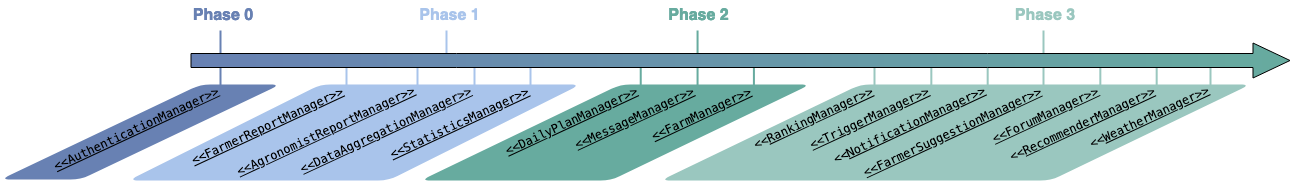
\includegraphics[width=\textwidth]{../images_diagrams/dd/implementation_phases.png}
\caption{Implementation Phases.}
\label{fig:implementationPhases}
\end{figure}

\subsubsection{Web Server}
\noindent
As stated in Section \ref{sect:cloudComponent} the web server component can be implemented using a commercial-off-the-shelf product that can receive and handle HTTP requests. This should be implemented early in the development stages in order to enable early testing of the application components. 

\subsection{Integration and Testing Plan} \label{sect:ITP}
\subsubsection{Continuous Integration}
\label{sect:CI}
\noindent
Due to the complexity and size of this effort, it is best to adopt a continuous integration methodology to ensure that integration and testing is exhaustive, thorough, and complete. Continuous integration enable on-going testing; each time new code is developed and pushed, the entire software undergoes a full suite of tests. This practice requires a lot of set-up and maintenance, but it is preferable in order to successfully integrate the system and catch errors early.\smallskip\\
\noindent
With CI, testing occurs frequently even with small increments of development. As such a cadence, developers can find and address code and integration errors early in the development process. This does, however, mean that whenever new components are developed, the corresponding test modules need to be developed in parallel to support CI. This model tightly couples the implementation and the test phases of the development.

\subsubsection{System Testing}
As explained in Section \ref{sect:CI}, the system will continuously undergo testing as the implementation progresses. This lightens the load of final system testing. Once the system has been fully implemented and integrated with the CI testing model, the system will have undergone and passed all the CI tests as a whole. The final system testing phase would simply be a final validation of the system; to ensure that the system successfully meets the customer's expectations. 